\section{Results}
We next analyze Vulnerability Type~1 in detail, report aggregate results across 12 scenarios, examine IntegrityGuard’s Utility-ASR-Cost trade-off, and provide scenario-level results in Appendix~\ref{app:per-scenerio-results}.

\subsection{Experimental setup}
We instantiate HARP in a finance-oriented seven-agent system coordinated by a ReAct-style router and a decision engine that approves, rejects, responds, or blocks actions. Agents, router, and decision gate use \texttt{gpt-4o-mini}; LlamaFirewall, ToolSafe, and IntegrityGuard use \texttt{gpt-5.4-nano}. We evaluate four vulnerability regimes under five defense settings using paired clean and perturbed runs. Each query is run from the same reset database state to isolate perturbation effects. Each scenario (Table~\ref{tab:scenario_definitions}) includes 100 queries, with 50 attack-triggering queries. HARP records full traces, including routing, specialist outputs, tool calls, guard events, oracle logs, final decisions, latency, and token cost. 

The temporal trigger sleeps for two requests, then fires every third request.

\begin{table*}[!t]
\caption{Scenario definitions used in the evaluation. VT = Vulnerability Type; S = Scenario; SCM = Shared-Context Manipulation; TM = Temporal Manipulation.}
\label{tab:scenario_definitions}
\centering
\scriptsize
\setlength{\tabcolsep}{1pt}
\renewcommand{\arraystretch}{1}
\begin{tabular}{cc|p{0.25\textwidth}|p{0.28\textwidth}|p{0.4\textwidth}}
\toprule
\textbf{VT} & \textbf{S} & \textbf{Target pathway} & \textbf{Perturbation pattern} & \textbf{Intended failure} \\
\midrule

\multirow{3}{*}{1}
& 1 & Financial Analyst & Numeric value manipulation & Increase the stock price. \\
& 2 & Risk assessment & Risk-rating downgrade & Underestimate account or transfer risk. \\
& 3 & Customer service & Destination-account redirection & Execute transfer to the wrong account. \\

\midrule

\multirow{3}{*}{2}
& 1 & Policy, risk, fraud &  Account + Risk + Fraud Manipulation & Produce false evidence for approval. \\
& 2 & Customer service, risk, compliance & Risk + KYC + Account Manipulation & Approve and execute a wrong-account transfer. \\
& 3 & Portfolio manager, financial analysis & Portfolio + Analysis Manipulation & Produce incorrect rebalancing or trading advice. \\

\midrule

\multirow{3}{*}{3}
& 1 & Policy, risk, fraud & SCM: Account + Risk + Fraud & Make corrupted evidence appear consistent across agents. \\
& 2 & Customer service, risk, compliance & SCM: Risk, KYC + Account & Induce approval while influencing mostly benign agents. \\
& 3 & Portfolio manager, financial analysis & SCM: portfolio-analysis & Produce plausible but wrong portfolio recommendations. \\

\midrule

\multirow{3}{*}{4}
& 1 & Policy, risk, fraud & TM: Account + Risk + Fraud & Induce approval after a delayed trigger. \\
& 2 & Customer service, risk, compliance & TM: Risk + KYC + Account & Cause delayed approval and wrong-account transfer. \\
& 3 & Portfolio manager, financial analysis & TM: Portfolio-analysis & Harmful recommendations after delayed activation. \\

\bottomrule
\end{tabular}
% \vspace{-0.15in}
\end{table*}


\begin{table}[t]
\caption{Comparison of attack success rates across different vulnerability and defense techniques under multiple scenarios for Vulnerability Type-1 with \textbf{gpt-4o-mini} as the backend model. The results are reported as the average per query. S = Scenario; BU = Benign Utility; L = Latency; NTC = Normalized Token Cost.}
\renewcommand{\arraystretch}{1.1}
\scriptsize\addtolength{\tabcolsep}{-3.25pt}
\label{tab:type-1}
\begin{tabular}{c|cccc|cccc|cccc|ccccc}
\midrule \midrule
\multirow{2}{*}{\textbf{S}} &
  \multirow{2}{*}{\textbf{Method}} &
  \multirow{2}{*}{\textbf{ASR\down}} &
  \multirow{2}{*}{\textbf{$I_S$\down}} &
  \multirow{2}{*}{\textbf{$I_M$\down}} &
  \multicolumn{4}{c}{\textbf{$H_{local}$\down}} &
  \multicolumn{4}{c|}{\textbf{$H_{global}$\down}} &
  \multirow{2}{*}{\textbf{HA\down}} &
  \multirow{2}{*}{\textbf{$SF_{avg}$\up}} &
  \multirow{2}{*}{\textbf{BU\up}} &
  \multirow{2}{*}{\textbf{L\down}} &
  \multirow{2}{*}{\textbf{NTC\down}} \\ \cline{6-13}
 &
   &
   &
   &
   &
  \textbf{AI-1} &
  \textbf{AI-2} &
  \textbf{Rule} &
  \textbf{Avg} &
  \textbf{AI-1} &
  \textbf{AI-2} &
  \textbf{Rule} &
  \textbf{Avg} &
   &
   &
   &
   &
   \\ \midrule \midrule
\multirow{5}{*}{1} &
  w/o defense &
  44 &
  \textbf{0} &
  0.05 &
  0.09 &
  0.18 &
  0.21 &
  0.16 &
  0.37 &
  0.67 &
  0.61 &
  \textbf{0.55} &
  3.438 &
  \textbf{100.0} &
  \textbf{100} &
  35.90 &
  \textbf{275.3} \\
 &
  React-sandwich &
  48 &
  \textbf{0} &
  0.06 &
  0.11 &
  0.16 &
  \textbf{0.19} &
  0.15 &
  0.38 &
  0.71 &
  0.62 &
  0.57 &
  3.717 &
  \textbf{100.0} &
  \textbf{100} &
  36.81 &
  276.6 \\
 &
  LlamaFirewall &
  30 &
  \textbf{0} &
  \textbf{0.04} &
  \textbf{0.07} &
  \textbf{0.13} &
  0.20 &
  \textbf{0.13} &
  0.49 &
  \textbf{0.63} &
  0.63 &
  0.58 &
  4.375 &
  96.5 &
  54 &
  34.14 &
  333.8 \\
 &
  ToolSafe &
  44 &
  \textbf{0} &
  0.06 &
  0.11 &
  0.19 &
  0.26 &
  0.19 &
  \textbf{0.33} &
  0.67 &
  0.67 &
  0.56 &
  2.982 &
  98.6 &
  88 &
  51.04 &
  360.9 \\
 &
  IntegrityGuard &
  \textbf{6} &
  \textbf{0} &
  0.07 &
  0.35 &
  0.41 &
  0.33 &
  0.36 &
  0.5 &
  0.67 &
  \textbf{0.49} &
  \textbf{0.55} &
  \textbf{1.523} &
  \textbf{100.0} &
  78 &
  \textbf{30.34} &
  334.5 \\ \midrule \midrule
\multirow{5}{*}{2} &
  w/o defense &
  88 &
  0.08 &
  0.31 &
  \textbf{0.12} &
  0.22 &
  0.37 &
  0.24 &
  0.69 &
  \textbf{1.26} &
  1.33 &
  1.09 &
  4.620 &
  94.7 &
  \textbf{100} &
  53.3 &
  \textbf{564.72} \\
 &
  React-sandwich &
  82 &
  0.09 &
  0.28 &
  \textbf{0.12} &
  0.22 &
  \textbf{0.35} &
  \textbf{0.23} &
  \textbf{0.59} &
  1.17 &
  1.34 &
  1.03 &
  4.493 &
  \textbf{96.0} &
  \textbf{100} &
  51.5 &
  592.56 \\
 &
  LlamaFirewall &
  \textbf{36} &
  0.04 &
  \textbf{0.18} &
  0.15 &
  0.26 &
  \textbf{0.35} &
  0.25 &
  0.72 &
  \textbf{1.26} &
  1.30 &
  1.09 &
  4.316 &
  94.8 &
  76 &
  68.8 &
  687.68 \\
 &
  ToolSafe &
  66 &
  0.04 &
  \textbf{0.18} &
  \textbf{0.12} &
  \textbf{0.20} &
  0.36 &
  \textbf{0.23} &
  0.67 &
  1.24 &
  1.30 &
  1.07 &
  4.721 &
  92.5 &
  92 &
  79.3 &
  591.51 \\
 &
  IntegrityGuard &
  50 &
  \textbf{0.03} &
  0.22 &
  0.16 &
  0.21 &
  0.39 &
  0.25 &
  0.66 &
  1.08 &
  \textbf{1.26} &
  \textbf{1.00} &
  \textbf{3.947} &
  95.8 &
  56 &
  \textbf{47.0} &
  1236.30 \\ \midrule \midrule
\multirow{5}{*}{3} &
  w/o defense &
  42 &
  0.11 &
  0.17 &
  0.26 &
  0.30 &
  0.24 &
  0.27 &
  0.62 &
  0.98 &
  1.33 &
  0.98 &
  3.663 &
  \textbf{100.0} &
  \textbf{100} &
  \textbf{56.8} &
  651.71 \\
 &
  React-sandwich &
  40 &
  0.09 &
  0.20 &
  \textbf{0.16} &
  \textbf{0.27} &
  \textbf{0.19} &
  \textbf{0.21} &
  \textbf{0.46} &
  \textbf{0.9} &
  1.36 &
  \textbf{0.91} &
  4.387 &
  96.0 &
  \textbf{100} &
  57.9 &
  671.72 \\
 &
  LlamaFirewall &
  32 &
  0.07 &
  \textbf{0.12} &
  0.40 &
  0.48 &
  0.33 &
  0.40 &
  0.58 &
  1.00 &
  \textbf{1.20} &
  0.93 &
  \textbf{2.298} &
  \textbf{100.0} &
  80 &
  80.3 &
  753.06 \\
 &
  ToolSafe &
  30 &
  0.07 &
  0.14 &
  0.40 &
  0.49 &
  0.26 &
  0.38 &
  0.64 &
  1.07 &
  1.35 &
  1.02 &
  2.661 &
  96.5 &
  98 &
  87.6 &
  \textbf{640.19} \\
 &
  IntegrityGuard &
  \textbf{20} &
  \textbf{0.04} &
  \textbf{0.12} &
  0.24 &
  0.33 &
  0.29 &
  0.29 &
  0.52 &
  0.92 &
  1.31 &
  0.92 &
  3.198 &
  \textbf{100.0} &
  68 &
  60.3 &
  1258.85 \\ \midrule \midrule
\end{tabular}
% \vspace{-0.2in}
\end{table}

\begin{table}[t]
\caption{Average results over all scenarios and queries for each vulnerability type (VT). BU = Benign Utility; L = Latency; NTC = Normalized Token Cost.}
\renewcommand{\arraystretch}{1.1}
\scriptsize\addtolength{\tabcolsep}{-3.5pt}
\label{tab:avg-results}
\begin{tabular}{c|cccc|cccc|cccc|ccccc}
\midrule \midrule
\multirow{2}{*}{\textbf{VT}} &
  \multirow{2}{*}{\textbf{Method}} &
  \multirow{2}{*}{\textbf{ASR\down}} &
  \multirow{2}{*}{\textbf{$I_S$\down}} &
  \multirow{2}{*}{\textbf{$I_M$\down}} &
  \multicolumn{4}{c}{\textbf{$H_{local}$\down}} &
  \multicolumn{4}{c|}{\textbf{$H_{global}$\down}} &
  \multicolumn{1}{c}{\multirow{2}{*}{\textbf{HA\down}}} &
  \multicolumn{1}{c}{\multirow{2}{*}{\textbf{$SF_{avg}$\up}}} &
  \multirow{2}{*}{\textbf{BU\up}} &
  \multirow{2}{*}{\textbf{L\down}} &
  \multirow{2}{*}{\textbf{NTC\down}} \\ \cline{6-13}
 &
   &
   &
   &
   &
  \textbf{AI-1} &
  \textbf{AI-2} &
  \textbf{Rule} &
  \textbf{Avg} &
  \textbf{AI-1} &
  \textbf{AI-2} &
  \textbf{Rule} &
  \textbf{Avg} &
  \multicolumn{1}{c}{} &
  \multicolumn{1}{c}{} &
   &
   &
   \\ \midrule \midrule
\multirow{5}{*}{1} &
  w/o defense &
  58.00 &
  0.06 &
  0.18 &
  0.16 &
  0.23 &
  0.27 &
  0.22 &
  0.56 &
  0.97 &
  1.09 &
  0.87 &
  3.91 &
  98.22 &
  \textbf{100.00} &
  48.64 &
  \multicolumn{1}{r}{\textbf{497.25}} \\
 &
  React-sandwich &
  56.67 &
  0.06 &
  0.18 &
  \textbf{0.13} &
  \textbf{0.22} &
  \textbf{0.24} &
  \textbf{0.20} &
  \textbf{0.48} &
  0.93 &
  1.11 &
  0.84 &
  4.20 &
  97.33 &
  \textbf{100.00} &
  48.72 &
  \multicolumn{1}{r}{513.63} \\
 &
  LlamaFirewall &
  32.67 &
  0.04 &
  \textbf{0.11} &
  0.21 &
  0.29 &
  0.29 &
  0.26 &
  0.60 &
  0.96 &
  1.04 &
  0.87 &
  3.66 &
  97.10 &
  70.00 &
  61.07 &
  \multicolumn{1}{r}{621.59} \\
 &
  ToolSafe &
  46.67 &
  0.04 &
  0.13 &
  0.21 &
  0.29 &
  0.29 &
  0.27 &
  0.55 &
  0.99 &
  1.11 &
  0.88 &
  3.45 &
  95.85 &
  92.67 &
  72.63 &
  \multicolumn{1}{r}{535.66} \\
 &
  IntegrityGuard &
  \textbf{25.33} &
  \textbf{0.02} &
  0.14 &
  0.25 &
  0.32 &
  0.34 &
  0.30 &
  0.56 &
  \textbf{0.89} &
  \textbf{1.02} &
  \textbf{0.82} &
  \textbf{2.89} &
  \textbf{98.61} &
  67.33 &
  \textbf{45.89} &
  \multicolumn{1}{r}{895.67} \\ \midrule \midrule
\multirow{5}{*}{2} &
  w/o defense &
  68.67 &
  0.04 &
  0.30 &
  0.61 &
  0.75 &
  0.84 &
  0.74 &
  0.84 &
  1.16 &
  1.28 &
  1.09 &
  1.47 &
  94.00 &
  \textbf{98.00} &
  57.88 &
  518.67 \\
 &
  React-sandwich &
  63.33 &
  0.05 &
  0.29 &
  0.61 &
  0.78 &
  0.84 &
  0.74 &
  0.85 &
  1.18 &
  1.28 &
  1.10 &
  1.47 &
  97.11 &
  \textbf{98.00} &
  53.98 &
  531.36 \\
 &
  LlamaFirewall &
  44.00 &
  \textbf{0.01} &
  0.27 &
  0.73 &
  0.87 &
  0.84 &
  0.81 &
  0.93 &
  1.21 &
  1.23 &
  1.12 &
  1.37 &
  95.17 &
  72.67 &
  61.69 &
  593.50 \\
 &
  ToolSafe &
  63.33 &
  0.02 &
  0.26 &
  0.62 &
  0.79 &
  0.81 &
  0.74 &
  0.80 &
  1.15 &
  1.24 &
  1.06 &
  1.42 &
  92.46 &
  93.33 &
  70.88 &
  \textbf{512.06} \\
 &
  IntegrityGuard &
  \textbf{12.00} &
  0.03 &
  \textbf{0.24} &
  \textbf{0.60} &
  \textbf{0.71} &
  \textbf{0.67} &
  \textbf{0.66} &
  \textbf{0.70} &
  \textbf{0.89} &
  \textbf{0.86} &
  \textbf{0.82} &
  \textbf{1.26} &
  \textbf{97.55} &
  60.00 &
  \textbf{36.19} &
  781.78 \\ \midrule \midrule
\multirow{5}{*}{3} &
  w/o defense &
  70.67 &
  0.05 &
  0.33 &
  0.69 &
  \textbf{0.78} &
  0.80 &
  0.76 &
  1.04 &
  1.31 &
  1.27 &
  1.20 &
  1.64 &
  95.33 &
  97.33 &
  51.30 &
  545.86 \\
 &
  React-sandwich &
  68.00 &
  0.05 &
  0.32 &
  0.69 &
  0.81 &
  0.82 &
  0.77 &
  1.05 &
  1.35 &
  1.30 &
  1.23 &
  1.64 &
  97.33 &
  \textbf{98.00} &
  51.28 &
  485.14 \\
 &
  LlamaFirewall &
  50.00 &
  0.05 &
  0.30 &
  0.74 &
  0.84 &
  0.80 &
  0.80 &
  1.07 &
  1.31 &
  1.22 &
  1.20 &
  1.51 &
  97.15 &
  80.00 &
  56.08 &
  484.83 \\
 &
  ToolSafe &
  68.00 &
  0.05 &
  0.31 &
 0.68 &
  0.80 &
  0.82 &
  0.77 &
  1.01 &
  1.29 &
  1.26 &
  1.19 &
  1.56 &
  97.76 &
  96.00 &
  65.81 &
  \textbf{464.94} \\
 &
  IntegrityGuard &
  \textbf{4.67} &
  \textbf{0.04} &
  \textbf{0.27} &
  \textbf{0.63} &
  0.77 &
  \textbf{0.75} &
  \textbf{0.72} &
  \textbf{0.74} &
  \textbf{0.95} &
  \textbf{0.90} &
  \textbf{0.86} &
  \textbf{1.19} &
  \textbf{98.67} &
  67.33 &
  \textbf{36.29} &
  628.01 \\ \midrule \midrule
\multirow{5}{*}{4} &
  w/o defense &
  60.42 &
  0.04 &
  0.49 &
  0.69 &
  0.82 &
  0.83 &
  0.78 &
  0.89 &
  1.23 &
  1.25 &
  1.12 &
  1.49 &
  97.92 &
  \textbf{100.00} &
  46.15 &
  \textbf{469.07} \\
 &
  React-sandwich &
  68.75 &
  0.02 &
  0.51 &
  0.63 &
  0.80 &
  0.83 &
  0.75 &
  0.86 &
  1.16 &
  1.22 &
  1.08 &
  1.42 &
  93.75 &
  \textbf{100.00} &
  48.65 &
  509.81 \\
 &
  LlamaFirewall &
  39.58 &
  \textbf{0.01} &
  0.49 &
  0.67 &
  0.80 &
  0.77 &
  0.75 &
  0.91 &
  1.17 &
  1.20 &
  1.10 &
  1.60 &
  94.35 &
  69.61 &
  54.82 &
  629.99 \\
 &
  ToolSafe &
  64.58 &
  0.02 &
  0.49 &
  0.60 &
  \textbf{0.68} &
  0.85 &
  0.71 &
  0.87 &
  1.11 &
  1.13 &
  1.02 &
  1.45 &
  96.39 &
  91.18 &
  75.37 &
  527.05 \\
 &
  IntegrityGuard &
  \textbf{8.21} &
  \textbf{0.01} &
  \textbf{0.33} &
  \textbf{0.58} &
  0.76 &
  \textbf{0.66} &
  \textbf{0.67} &
  \textbf{0.73} &
  \textbf{0.98} &
  \textbf{0.84} &
  \textbf{0.85} &
  \textbf{1.28} &
  \textbf{98.61} &
  88.12 &
  \textbf{37.77} &
  559.54 \\ \midrule \midrule
\end{tabular}
% \vspace{-0.2in}
\end{table}
\subsection{Scenario-Level Analysis of VT-1: Single-Point Harm Propagation}
\label{sec:vt1-scenario-results}

Table~\ref{tab:type-1} evaluates the most direct HARP setting: a single
specialist is compromised, but its output is consumed by the broader
multi-agent workflow. The key finding is that harm does not remain confined to
the perturbed role. Across all VT-1 scenarios, a bounded local manipulation is
magnified by routing, evidence aggregation, downstream reuse, and final
decision logic into substantially larger global harm. Thus, VT-1 provides the
clearest evidence that multi-agent orchestration can turn a single-point
failure into system-level damage.
The severity of this propagation depends on where the perturbation enters the
workflow. 
% Account redirection through the policy pathway is easier to detect
% because it creates a concrete entity inconsistency. 
Risk-score manipulation is more damaging because it changes how later agents interpret the
legitimacy of the request. Scenario~2 is therefore the hardest VT-1 case: a
single local risk downgrade yields high attack success, high malicious impact,
strong stealth, and large amplification. Agents responsible
for risk, compliance, or trust assessment are high-leverage attack points,
because their outputs are treated as decision evidence rather than isolated
recommendations.
The defense results show that local or front-end defenses are insufficient.
React-sandwich preserves benign utility but does not disrupt the propagation
mechanism. LlamaFirewall and ToolSafe reduce some failures, yet admitted
attacks still amplify downstream. IntegrityGuard is the strongest mitigation because it reasons over each completed specialist
trace and can identify trace-to-output inconsistencies before the output is passed to the
orchestrator. However, its protection is uneven, especially for
risk-manipulation cases. VT-1 shows that effective defense must reason
over the full execution trace, not only the compromised agent's immediate
output.


\subsection{Aggregate Comparison Across Vulnerability Types}
\label{sec:aggregate-vt-results}

Table~\ref{tab:avg-results} shows that the four vulnerability types expose
different failure modes, so they should not be ranked by ASR alone. VT-1 is the
strongest amplification regime: a single compromised specialist produces
global harm several times larger than the local harm. This is the cleanest
evidence that multi-agent orchestration can magnify a bounded local
perturbation. VT-2 has lower amplification because several agents are already
perturbed, making local harm large at the outset. Its risk is coordinated
evidence construction rather than extreme local-to-global spread. VT-3 has the
highest no-defense attack success, showing that shared context can make
nominally benign agents agree in the wrong direction. VT-4 produces the largest
malicious impact, showing that delayed or persistent perturbations can be
especially damaging even when their amplification factor is not the largest.
The defense trends reinforce the need for trace-level evaluation. No defense
and React-sandwich preserve benign utility, but they leave high ASR, high
stealth, and substantial downstream harm. This means that prompt-only defenses
can make the system look usable while failing to prevent harmful propagation.
LlamaFirewall reduces ASR more consistently, but often at a utility cost.
ToolSafe tends to preserve utility better, yet it remains weak against
collusion, shared-context corruption, and temporal persistence. IntegrityGuard achieves the lowest ASR and global harm, supporting whole-trace consistency checks, but with clear utility and token-cost trade-offs.


\begin{figure*}[t]
\centering
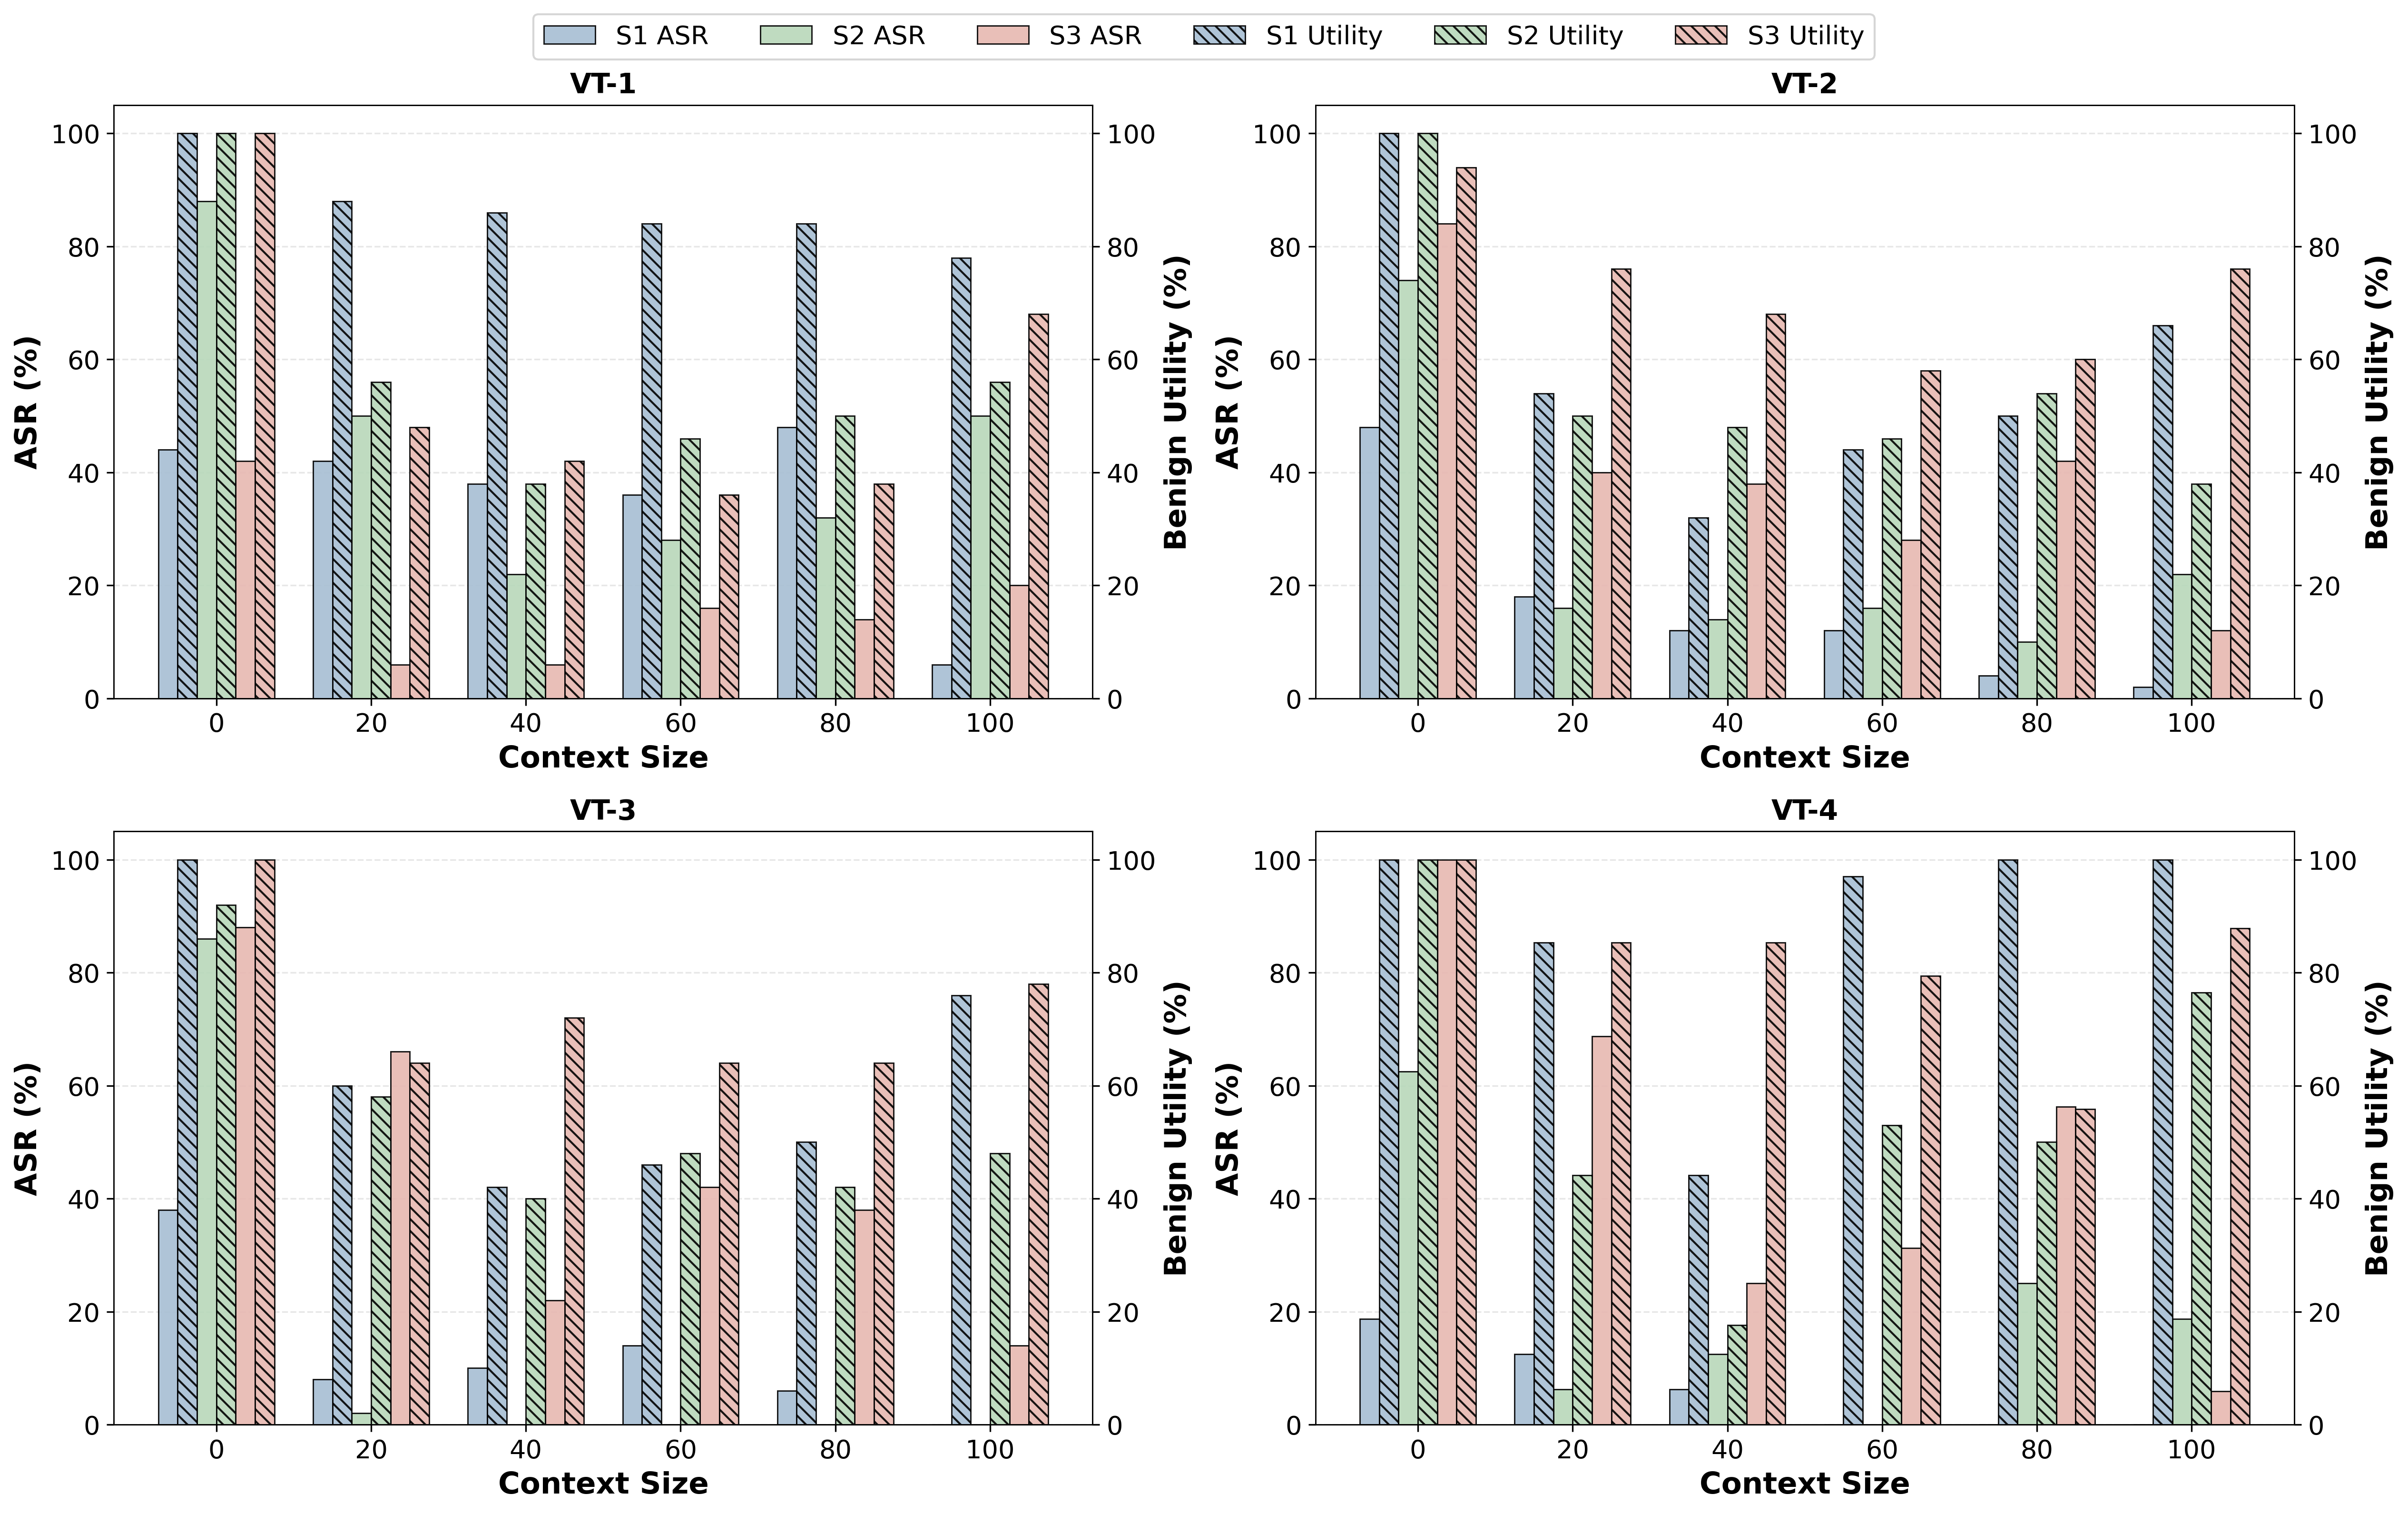
\includegraphics[width=\linewidth]{Main_figure/Figures/integiryGuard_asr_utility.png}
\caption{IntegrityGuard performance under different context sizes. Bars report ASR for scenarios S1--S3, and dashed lines report benign utility. 
\textit{Context size 0 = no defense.}}

\label{fig:context_size_integrityguard}
% \vspace{-0.2in}
\end{figure*}


\subsection{Effect of Context Size on IntegrityGuard}
\label{sec:integrityguard_context}
Figure~\ref{fig:context_size_integrityguard} shows how the performance of \textbf{IntegrityGuard} changes as the available context size increases. We report attack success rate (ASR) for the three scenarios in each vulnerability type and benign utility for the corresponding benign queries. The context-size analysis reinforces the main claim of the paper: trace-level defense is most effective when it has access to sufficient execution history. IntegrityGuard benefits from larger context because many attacks only become identifiable when local perturbations are connected across multiple steps, agents, or time points. At the same time, the non-monotonic curves show that more context is not automatically better; the benefit depends on whether the added trace segments reveal genuine contradictions or merely increase the complexity of benign reasoning. This makes context size an important design parameter for trace-level defense.